\documentclass[11pt, oneside]{article}   	% use "amsart" instead of "article" for AMSLaTeX format
\usepackage{geometry}                		% See geometry.pdf to learn the layout options. There are lots.
\geometry{letterpaper}                   		% ... or a4paper or a5paper or ... 
%\geometry{landscape}                		% Activate for rotated page geometry
\usepackage[parfill]{parskip}    		% Activate to begin paragraphs with an empty line rather than an indent
\usepackage{graphicx}				% Use pdf, png, jpg, or eps§ with pdflatex; use eps in DVI mode
								% TeX will automatically convert eps --> pdf in pdflatex		
\usepackage{amssymb}
\usepackage{amsmath}
\DeclareMathOperator*{\argmax}{argmax} % create argmax command
\usepackage{booktabs}
\usepackage[procnames]{listings}
\usepackage{color}
\title{Practical 4:\\
 Learning to Play Swingy Monkey}
\author{Samuel Daulton, Taylor Killian, and Andrew Petschek (ML Marauders)}
%\date{}							% Activate to display a given date or no date

\begin{document}
\maketitle
\section{Technical Approach}
In this practical we were tasked with creating a learning agent to achieve a high score in the game Swingy Monkey. The goal of Swingy Monkey is to pass (by dodging) as many tree trunks as possible without flying off the screen upwards or downwards, or swinging/jumping into the tree which results in a game over.  The monkey has two actions: jump to a new vine (at a random height above) or swing on the current vine. The location of the gap in each tree trunk is random, as is the gravity of each game.  We were provided with code for the Swingy Monkey game and additional code for retrieving information from the game at each time step.  Specifically, we were provided with a Python dictionary containing the following:
\begin{verbatim}
{'score':<current score>,
'tree':{
    'dist':<pixels to next tree trunk>,
    'top': <height of top of tree trunk gap>,
    'bot': <height of bottom of tree trunk gap> },
'monkey': {
    'vel': <current monkey y-axis speed>,
    'top': <height of top of monkey>,
    'bot': <height of bottom of monkey> }}
\end{verbatim}
The reward for the previous time step is given to be:
$$
\text{Reward} =
\begin{cases}
1, & \text{for passing a tree trunk} \\
-10, & \text{for falling off the top or bottom of the screen}\\
-5, & \text{for hitting the tree}\\
0, & \text{otherwise}
\end{cases}
$$

In this section, we outline our methodology for setting up a routine for the computer to learn how to effectively play the Swingy Monkey game via reinforcement learning.  In particular, we specify the Markov decision process framework for the problem.  In subsequent sections, we outline two distinct reinforcement learning methodologies used to learn a policy capable of achieving high scores.  Both of our implemented methods attempt to approximate a function to estimate the Q-function under the assumption of a continuous state space. This learned Q-function is then used to derive the optimal policy the machine uses in future game play.

\subsection{Markov Decision Process (MDP) Specification}
To model Swingy Monkey as an MDP, we used the provided discrete reward function and actions as defined in Section 1.  The state space for our model is all possible tuples of the form:                                                                                                                                                                  
\noindent\begin{verbatim}
  (tree dist, tree top, tree bot, monkey vel, monkey top, monkey bot, gravity)
\end{verbatim}

It is important to note that the state space is assumed to be continuous.  This makes pre-computing explicit policies infeasible.  However, since there are a finite number of possible actions from any state we can compute the best action at each time step, given an estimation of the Q-function. Details about estimating the Q function are outlined in Section 3.

\subsection{Learning Gravity}
In the after the first time step of each game, the agent learns what the value of gravity by calculating the vertical distance that the monkey moves (when the monkey swings on its current vine).  Explicitly,
$$\text{gravity} = -|\text{monkeybot}_{0} - \text{monkeybot}_{1}|$$

Note that, for purposes of the game, gravity is a constant velocity.

\section{Approach 1: Epoch Iterated Q-Learning}
The first approach we took was using Epoch Iterated Q-learning, again using a Random Forest Regressor to infer the Q-function.  The primary motivation for using this method was that we wanted to account for the incremental knowledge gained after every epoch when training the machine. We proceeded to iteratively update our policy based on the previous game play in an online fashion. The methodology is as follows:
\begin{enumerate}
  \item Run 1 epoch where the agent takes random actions.
  \item Train a Random Forest Regressor using the state-action-reward dataset from the first epoch to infer the Q-function.  As in batch reinforcement learning, the Q-function will be used to compute the policy for a given state on-the-fly) using equation 1.
  \item Run 100 learning epochs.  In the first learning epoch, the agent takes a random action with a probability of .5 for each time step.  After every 10 epochs, the probability of an agent taking a random action is reduced by .05.  This is to ensure that the agent explores a lot at first and slowly transitions to exploiting the learned policy more as time goes on, until the agent chooses actions solely based on the determined policy.  After each epoch, we append the dataset from the most recent epoch to the aggregated dataset of all previous epochs (including the initial random epoch) and retrain a Random Forest Regressor using the entire dataset.  Using this Q-function, we obtain the updated policy using Equations (1) and (2).
 \item After training the best policy we run an additional 100 epochs with actions chosen according to that policy, removing any and all exploration. The results of this test of our policy comprise the results we report below in Section~\ref{sec:analysis}.
\end{enumerate}

\section{Approach 2: Batch Reinforcement Learning}
Our secondary approach was to use batch reinforcement learning to allow an agent to learn from the actions and rewards of a batch of epochs. We chose this approach due to our foundational assumption that the state space was continuous. With continuous states we wanted to gather as much training data as possible to approximate the Q-function. With batches of state, action and reward data, generated by the current policy provides we were able to train a more effective policy after each batch. The methodology is as follows:
\begin{enumerate}
  \item Run 1 batch of 100 epochs were the agent takes a random action at each timestep.  The purpose of this is to create an initial dataset where each observation in the dataset is of the form: (state, action) $\longrightarrow$ reward.
  \item Train a Random Forest Regressor using state and action as predictor variables and reward as the response variable.  This trained Random Forest is our Q-function.  For a given state and action, the Random Forest will return the expected value.
  \item In the next batch, we use this Q-function to determine what action to take at any given state.  It is important to note that we never pre-compute a policy $\pi$ over all states; rather, we compute the best action (to our knowledge) given we are in a particular state.  Specifically, at each timestep we compute policy for the current state, $s$, as follows:
\begin{align}
\pi(s) &= \argmax_{a\in A} Q(s,a)
\end{align}
where we solve the Bellman's equation, 
\begin{align}
Q(s,a) &= Q(s,a) + \alpha\left[R(s,a) + \gamma \max_{a'} Q(s,a') - Q(s,a)\right]
\end{align}
This is reasonable, computationally, since there are only two possible actions.  Despite computing $\pi^*(s)$ on-the-fly, we will still refer to $\pi^*$ as the policy.
  \item Run 20 optimization (i.e. learning) batches each consisting of 50 epochs, in which the agent takes a random action instead of following the policy with probability .1. The idea with the random actions is to explore 10\% of the time.  After each batch, append the dataset from the most recent batch to the aggregated dataset of all previous batches (including the initial random batch) and retrain a Random Forest Regressor using the entire dataset.  Hence, we update our Q-function to reflect what the agent has learned.  Using this Q-function, we again compute the policy for the current state on the fly.
  
 Note that we chose to use 50 epochs per learning batch to obtain a satisfactory balance between performance and runtime.

\item After training what we could consider $\pi^*$, we run a final batch to test the policy. We run an addition 100 epochs without any exploration. The results from this test run provide the values we reported for this method in Section~\ref{sec:analysis}
 
\end{enumerate}

\section{Analysis of Methods}
\label{sec:analysis}

  \begin{center}
    Statistics from a Test Batch of 100 Epochs\\
      \vspace{3mm}
    \begin{tabular}{ | c | c | c | c | } 
      \hline
      Method & Mean & Min & Max \\ 
      \hline
      Batch RL & 8.51 & 0 & 82.51 \\ 
      \hline
      Epoch Iterated Q Learning & 2.21 & 0 & 15 \\  
      \hline
      Random & .23 & 0 & 2 \\
      \hline
    \end{tabular}
  \end{center}
  \vspace{3mm}
  The above table contains a few measures of how good the a policy is.  The optimal policy from Batch RL and Epoch Iterated RL are compared to a baseline policy where the agent choses a random action at each time step.  Batch RL yields substantially higher mean and maximum scores than Epoch Iterated Q Learning and Random.  Epoch Iterated Q Learning is also better than random, but is substantially worse than Batch RL.  \\
  
  \subsection{Figures}
  \begin{figure}[ht!]
  \centering
  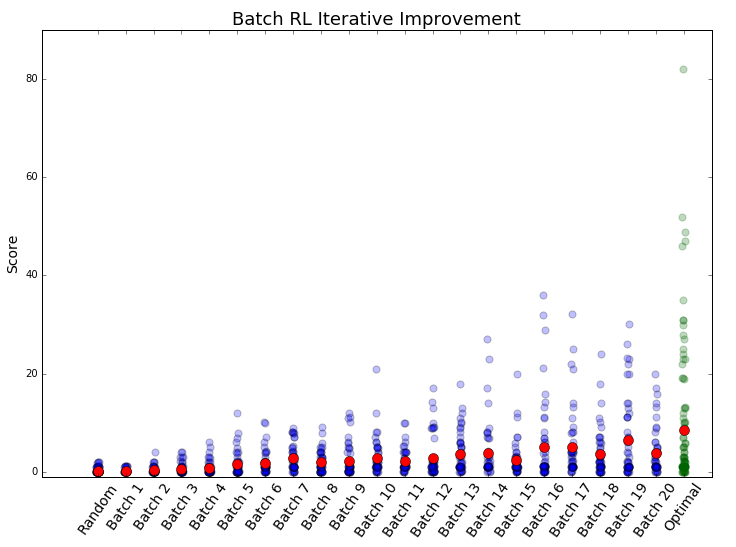
\includegraphics[width=0.95\textwidth]{batch_iterative_improvement}
  \caption{Plot of the distribution of scores for each batch.  The blue dots are scores from individual epochs of random (100 epochs) and learning batches (50 epochs each).  The green dots are scores from one batch of 100 epochs using the optimal policy.  Each red dot is the mean score of the corresponding batch.  Overall, batch reinforcement learning iteratively improves mean score}
   \end{figure}
  \begin{figure}[ht!]
  \centering
  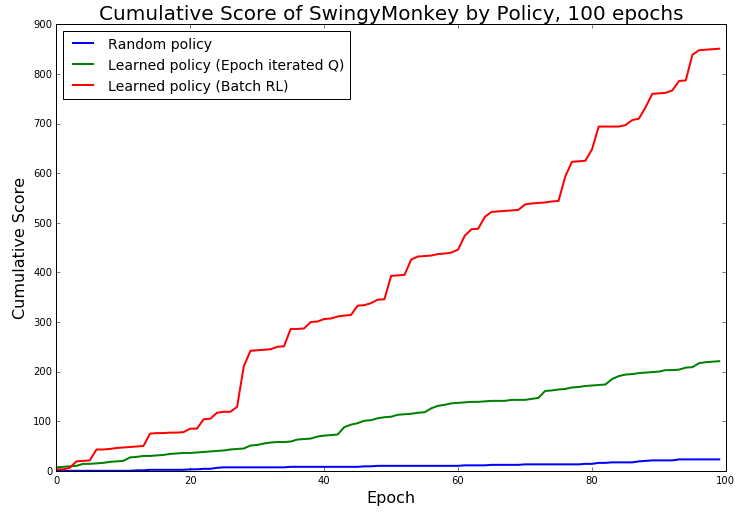
\includegraphics[width=0.95\textwidth]{cumulative_score}
  \caption{A plot of cumulative scores using the optimal policies from Batch RL and Epoch Iterated Q Learning.}
 \end{figure}  
 The large differences in maximum and mean scores between Batch RL and Epoch Iterated Q Learning probably comes from the disparity in the number of epochs that each is trained on.  We only run Epoch Iterated Q Learning for 100 epochs. We only ran Epoch Iterated Q Learning for 100 epochs because it is much more computationally expensive since we train a Random Forest Regressor after each epoch instead of after each batch.  

\section{Conclusion}
Batch RL works well for training agents to achieve high scores in Swingy Monkey.  Moreover, a policy optimized using Batch RL achieves substantially higher mean and maximum scores than a policy from Epoch Iterated Q Learning. We recognize that we made some assumptions that constrained our ability to achieve even better performance. Had we implemented \texttt{S,A,R,S,A} with Value Iteration we expect that our agent's learning would have been significantly more efficient and effective. In this discretized world, the policy is updated after every action, where our methodology needed to wait after several actions and decisions were made before updating the policy. These inefficiencies were readily apparent in the run-time of our algorithmic implementations and somewhat disappointing scores the agent was able to achieve. We understood the risks of making the modeling assumptions we made, that without much information about the environment and how the agent's actions affect its immediate reward we were limited in the type of performance gains that were possible. We were conservative in our approach and we received modest gains. We were however pleased that we did get the monkey to learn how to play the game and rack up a few great performances here and there. This was a really fun practical and are grateful that we got the chance to play video games as part of class.

Thanks for a great semester!

\end{document}  

